%\VignetteEngine{knitr}
%\VignetteIndexEntry{UV-radiation quantification with R: Catalogue of lamps}
%\VignetteDepends{knitr, photobiology, photobiologyLamps, photobiologygg, ggplot2}
%\VignetteKeyword{misc}

\documentclass{article}\usepackage[]{graphicx}\usepackage[]{color}
%% maxwidth is the original width if it is less than linewidth
%% otherwise use linewidth (to make sure the graphics do not exceed the margin)
\makeatletter
\def\maxwidth{ %
  \ifdim\Gin@nat@width>\linewidth
    \linewidth
  \else
    \Gin@nat@width
  \fi
}
\makeatother

\definecolor{fgcolor}{rgb}{0.345, 0.345, 0.345}
\newcommand{\hlnum}[1]{\textcolor[rgb]{0.686,0.059,0.569}{#1}}%
\newcommand{\hlstr}[1]{\textcolor[rgb]{0.192,0.494,0.8}{#1}}%
\newcommand{\hlcom}[1]{\textcolor[rgb]{0.678,0.584,0.686}{\textit{#1}}}%
\newcommand{\hlopt}[1]{\textcolor[rgb]{0,0,0}{#1}}%
\newcommand{\hlstd}[1]{\textcolor[rgb]{0.345,0.345,0.345}{#1}}%
\newcommand{\hlkwa}[1]{\textcolor[rgb]{0.161,0.373,0.58}{\textbf{#1}}}%
\newcommand{\hlkwb}[1]{\textcolor[rgb]{0.69,0.353,0.396}{#1}}%
\newcommand{\hlkwc}[1]{\textcolor[rgb]{0.333,0.667,0.333}{#1}}%
\newcommand{\hlkwd}[1]{\textcolor[rgb]{0.737,0.353,0.396}{\textbf{#1}}}%

\usepackage{framed}
\makeatletter
\newenvironment{kframe}{%
 \def\at@end@of@kframe{}%
 \ifinner\ifhmode%
  \def\at@end@of@kframe{\end{minipage}}%
  \begin{minipage}{\columnwidth}%
 \fi\fi%
 \def\FrameCommand##1{\hskip\@totalleftmargin \hskip-\fboxsep
 \colorbox{shadecolor}{##1}\hskip-\fboxsep
     % There is no \\@totalrightmargin, so:
     \hskip-\linewidth \hskip-\@totalleftmargin \hskip\columnwidth}%
 \MakeFramed {\advance\hsize-\width
   \@totalleftmargin\z@ \linewidth\hsize
   \@setminipage}}%
 {\par\unskip\endMakeFramed%
 \at@end@of@kframe}
\makeatother

\definecolor{shadecolor}{rgb}{.97, .97, .97}
\definecolor{messagecolor}{rgb}{0, 0, 0}
\definecolor{warningcolor}{rgb}{1, 0, 1}
\definecolor{errorcolor}{rgb}{1, 0, 0}
\newenvironment{knitrout}{}{} % an empty environment to be redefined in TeX

\usepackage{alltt}

\usepackage[utf8]{inputenc}
\usepackage{abbrev}
\usepackage[unicode=true,pdfusetitle,
 bookmarks=true,bookmarksnumbered=true,bookmarksopen=true,bookmarksopenlevel=2,
 breaklinks=false,pdfborder={0 0 1},backref=false,colorlinks=false]
 {hyperref}
\usepackage{listings}
\usepackage{booktabs}
\usepackage{breakurl}

\newcommand{\PB}{\textsf{photobiology}\xspace}
\newcommand{\PBVIS}{\textsf{photobiologyVIS}\xspace}
\newcommand{\PBUV}{\textsf{photobiologyUV}\xspace}
\newcommand{\PBPHY}{\textsf{photobiologyPhy}\xspace}
\newcommand{\PBCRY}{\textsf{photobiologyCry}\xspace}
\newcommand{\PBFil}{\textsf{photobiologyFilters}\xspace}
\newcommand{\PBLam}{\textsf{photobiologyLamps}\xspace}
\newcommand{\PBSen}{\textsf{photobiologySensors}\xspace}
\newcommand{\PBSun}{\textsf{photobiologySun}\xspace}
\IfFileExists{upquote.sty}{\usepackage{upquote}}{}

\begin{document}

\title{\PBSun Version 0.1.1\\ Catalogue of Solar Spectra}
\author{Pedro J. Aphalo}

\maketitle

\section{Introduction}

We will plot the emission spectra of the different lamps for which data is provided in the pacakge. We plot side-by-side the lamp output as spectral energy irradiance and as spectral photon irradiance. All spectra are normalized to an area of one under the whole curve.




\begin{knitrout}\footnotesize
\definecolor{shadecolor}{rgb}{0.969, 0.969, 0.969}\color{fgcolor}\begin{kframe}
\begin{alltt}
\hlkwd{library}\hlstd{(ggplot2)}
\hlkwd{library}\hlstd{(photobiology)}
\hlkwd{library}\hlstd{(photobiologyLamps)}
\hlkwd{library}\hlstd{(photobiologySun)}
\hlkwd{library}\hlstd{(photobiologygg)}
\end{alltt}


{\ttfamily\noindent\itshape\color{messagecolor}{\#\# Loading required package: proto\\\#\# Loading required package: splus2R\\\#\# Loading required package: plyr}}\end{kframe}
\end{knitrout}


We define a function to do the actual plotting so as to not repeat code, and to make changes easier in the future.

\begin{knitrout}\footnotesize
\definecolor{shadecolor}{rgb}{0.969, 0.969, 0.969}\color{fgcolor}\begin{kframe}
\begin{alltt}
\hlstd{lamp.plotter} \hlkwb{<-} \hlkwa{function}\hlstd{(}\hlkwc{lamp.name}\hlstd{,} \hlkwc{w.low} \hlstd{=} \hlnum{250}\hlstd{,} \hlkwc{w.high} \hlstd{=} \hlnum{900}\hlstd{,} \hlkwc{scaled} \hlstd{=} \hlstr{"peak"}\hlstd{) \{}
    \hlstd{w.length.out} \hlkwb{<-} \hlkwd{seq}\hlstd{(}\hlkwc{from} \hlstd{= w.low,} \hlkwc{to} \hlstd{= w.high,} \hlkwc{length.out} \hlstd{=} \hlnum{300}\hlstd{)}
    \hlstd{spectrum.data} \hlkwb{<-} \hlkwd{calc_lamp_output}\hlstd{(}\hlkwc{w.length.out} \hlstd{= w.length.out,} \hlkwc{lamp.name} \hlstd{= lamp.name,}
        \hlkwc{scaled} \hlstd{= scaled)}
    \hlstd{spectrum.data} \hlkwb{<-} \hlkwd{na.omit}\hlstd{(spectrum.data)}
    \hlstd{fig_energy} \hlkwb{<-} \hlkwd{ggplot}\hlstd{(}\hlkwd{aes}\hlstd{(}\hlkwc{x} \hlstd{= w.length,} \hlkwc{y} \hlstd{= s.e.irrad),} \hlkwc{data} \hlstd{= spectrum.data)} \hlopt{+}
        \hlkwd{xlim}\hlstd{(w.low, w.high)} \hlopt{+} \hlkwd{labs}\hlstd{(}\hlkwc{x} \hlstd{=} \hlstr{"Wavelength (nm)"}\hlstd{,} \hlkwc{y} \hlstd{=} \hlstr{"Spectral energy irradiance\textbackslash{}n(rel. units)"}\hlstd{,}
        \hlkwc{title} \hlstd{= lamp.name)} \hlopt{+} \hlkwd{geom_line}\hlstd{()} \hlopt{+} \hlkwd{stat_peaks}\hlstd{(}\hlkwc{ignore_threshold} \hlstd{=} \hlnum{0.33}\hlstd{,}
        \hlkwc{colour} \hlstd{=} \hlstr{"red"}\hlstd{,} \hlkwc{span} \hlstd{=} \hlnum{21}\hlstd{)}
    \hlstd{fig_photon} \hlkwb{<-} \hlkwd{ggplot}\hlstd{(}\hlkwd{aes}\hlstd{(}\hlkwc{x} \hlstd{= w.length,} \hlkwc{y} \hlstd{= s.q.irrad),} \hlkwc{data} \hlstd{= spectrum.data)} \hlopt{+}
        \hlkwd{xlim}\hlstd{(w.low, w.high)} \hlopt{+} \hlkwd{labs}\hlstd{(}\hlkwc{x} \hlstd{=} \hlstr{"Wavelength (nm)"}\hlstd{,} \hlkwc{y} \hlstd{=} \hlstr{"Spectral photon irradiance\textbackslash{}n(rel. units)"}\hlstd{,}
        \hlkwc{title} \hlstd{= lamp.name)} \hlopt{+} \hlkwd{geom_line}\hlstd{()} \hlopt{+} \hlkwd{stat_peaks}\hlstd{(}\hlkwc{ignore_threshold} \hlstd{=} \hlnum{0.33}\hlstd{,}
        \hlkwc{colour} \hlstd{=} \hlstr{"red"}\hlstd{,} \hlkwc{span} \hlstd{=} \hlnum{21}\hlstd{)}
    \hlkwd{print}\hlstd{(fig_energy)}
    \hlkwd{print}\hlstd{(fig_photon)}
\hlstd{\}}
\end{alltt}
\end{kframe}
\end{knitrout}


\newpage

\section{Extraterrestrial solar spectra}

\begin{knitrout}\footnotesize
\definecolor{shadecolor}{rgb}{0.969, 0.969, 0.969}\color{fgcolor}\begin{kframe}
\begin{alltt}
\hlstd{spectra} \hlkwb{<-} \hlkwd{c}\hlstd{(}\hlstr{"WMO_Wehrli_AM0"}\hlstd{,} \hlstr{"ASTM_E490_AM0"}\hlstd{,} \hlstr{"Gueymard_AM0"}\hlstd{)}
\hlkwa{for} \hlstd{(spc} \hlkwa{in} \hlstd{spectra) \{}
    \hlkwd{lamp.plotter}\hlstd{(}\hlkwc{lamp.name} \hlstd{= spc,} \hlkwc{w.low} \hlstd{=} \hlnum{200}\hlstd{,} \hlkwc{w.high} \hlstd{=} \hlnum{4000}\hlstd{)}
\hlstd{\}}
\end{alltt}
\end{kframe}

{\centering 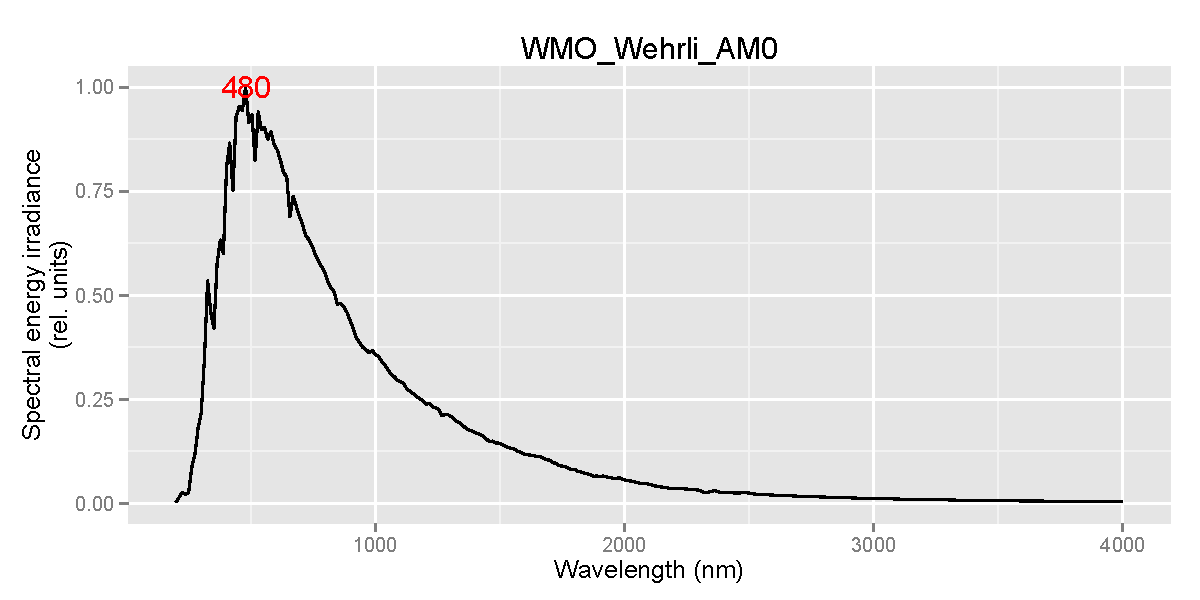
\includegraphics[width=.95\textwidth]{figure/pos-extraterrestrial1} 
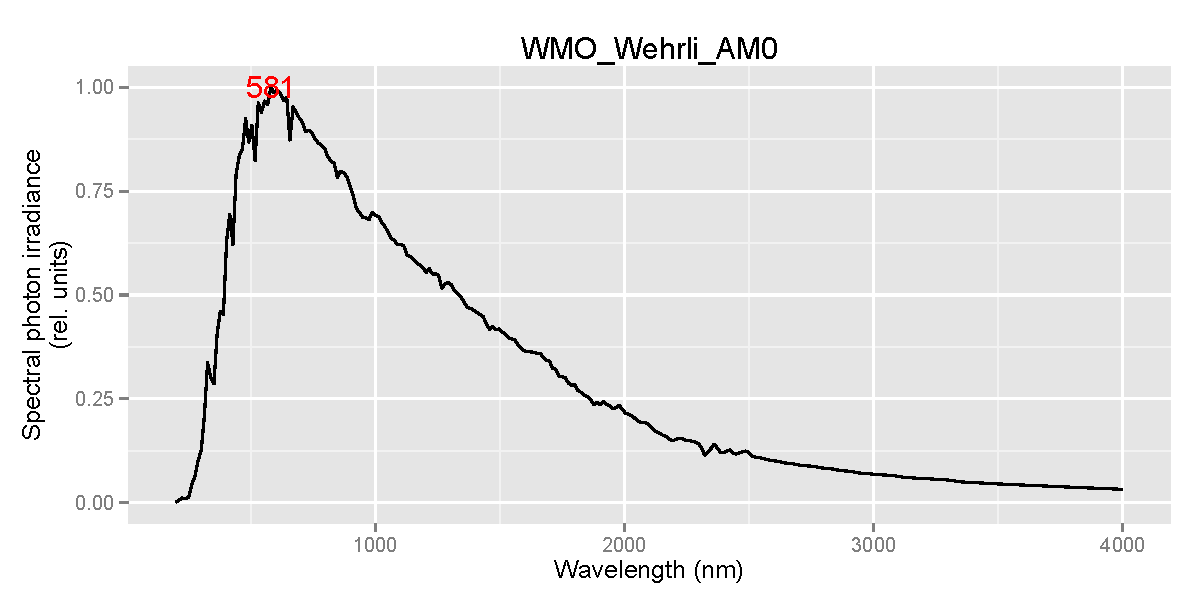
\includegraphics[width=.95\textwidth]{figure/pos-extraterrestrial2} 
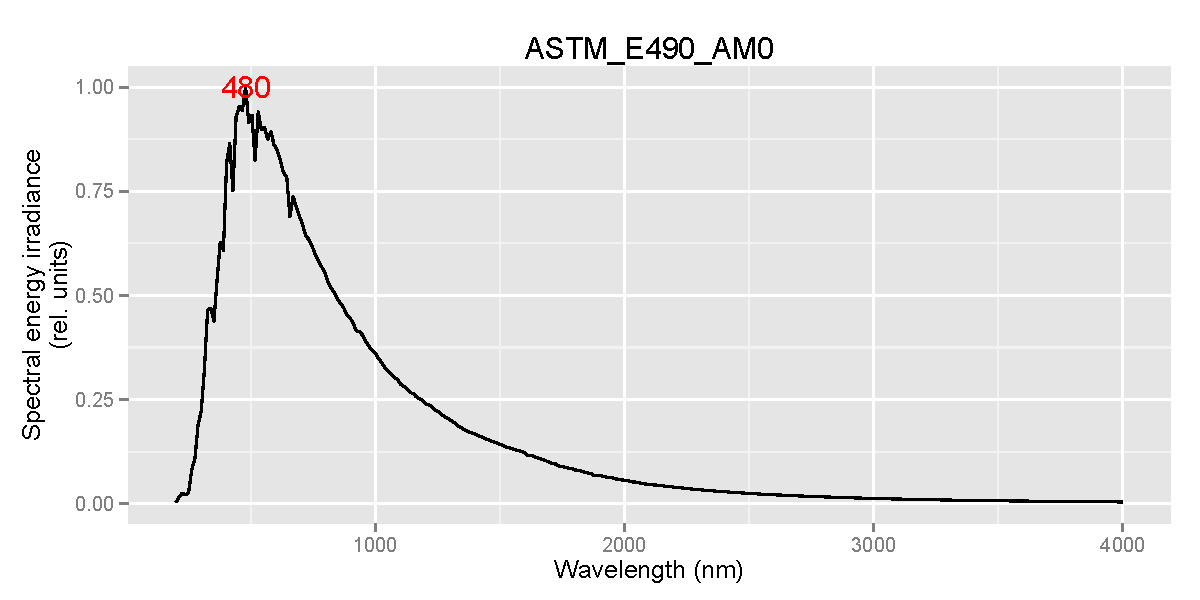
\includegraphics[width=.95\textwidth]{figure/pos-extraterrestrial3} 
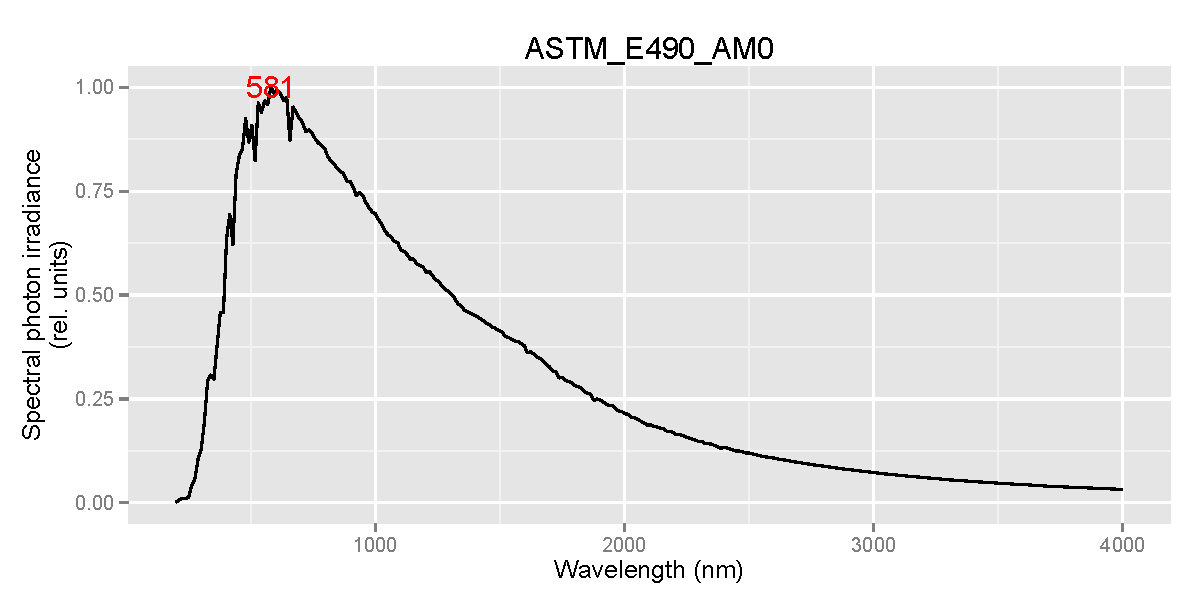
\includegraphics[width=.95\textwidth]{figure/pos-extraterrestrial4} 
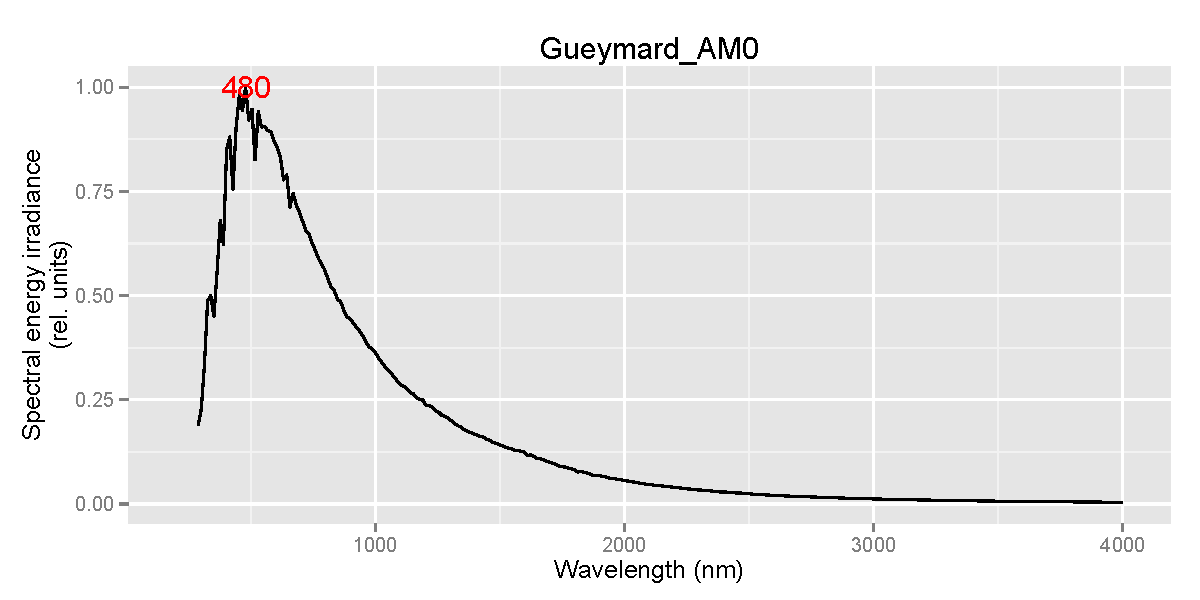
\includegraphics[width=.95\textwidth]{figure/pos-extraterrestrial5} 
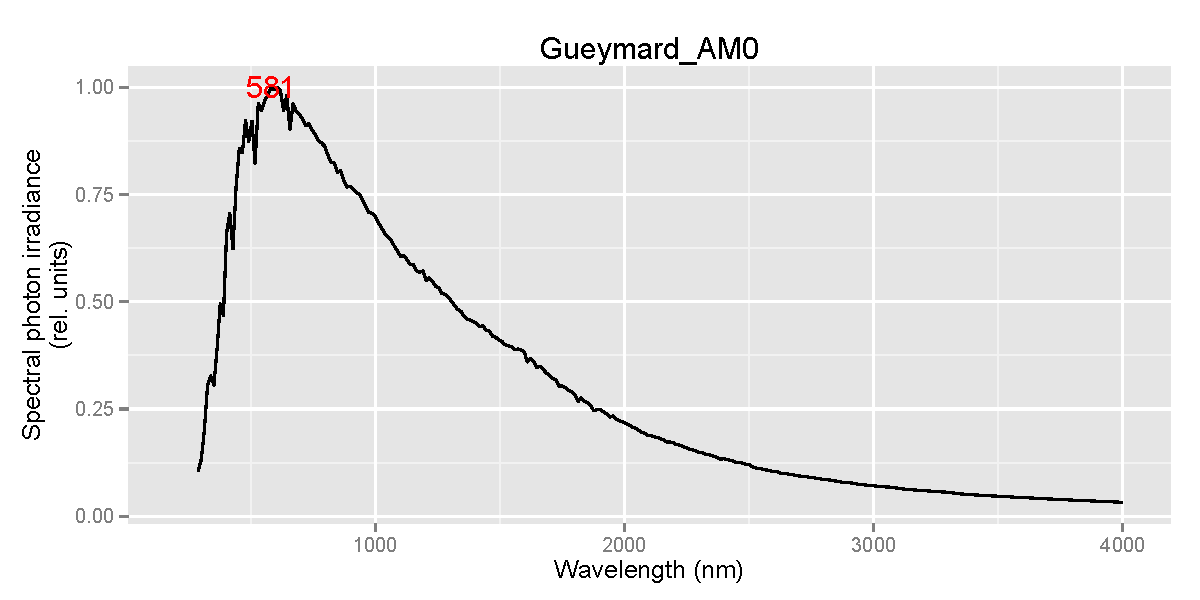
\includegraphics[width=.95\textwidth]{figure/pos-extraterrestrial6} 

}



\end{knitrout}


\section{Standard terrestrial solar spectra}

\begin{knitrout}\footnotesize
\definecolor{shadecolor}{rgb}{0.969, 0.969, 0.969}\color{fgcolor}\begin{kframe}
\begin{alltt}
\hlstd{spectra} \hlkwb{<-} \hlkwd{c}\hlstd{(}\hlstr{"ASTM_G173_direct"}\hlstd{,} \hlstr{"ASTM_G173_global"}\hlstd{)}
\hlkwa{for} \hlstd{(spc} \hlkwa{in} \hlstd{spectra) \{}
    \hlkwd{lamp.plotter}\hlstd{(}\hlkwc{lamp.name} \hlstd{= spc)}
\hlstd{\}}
\end{alltt}
\end{kframe}

{\centering 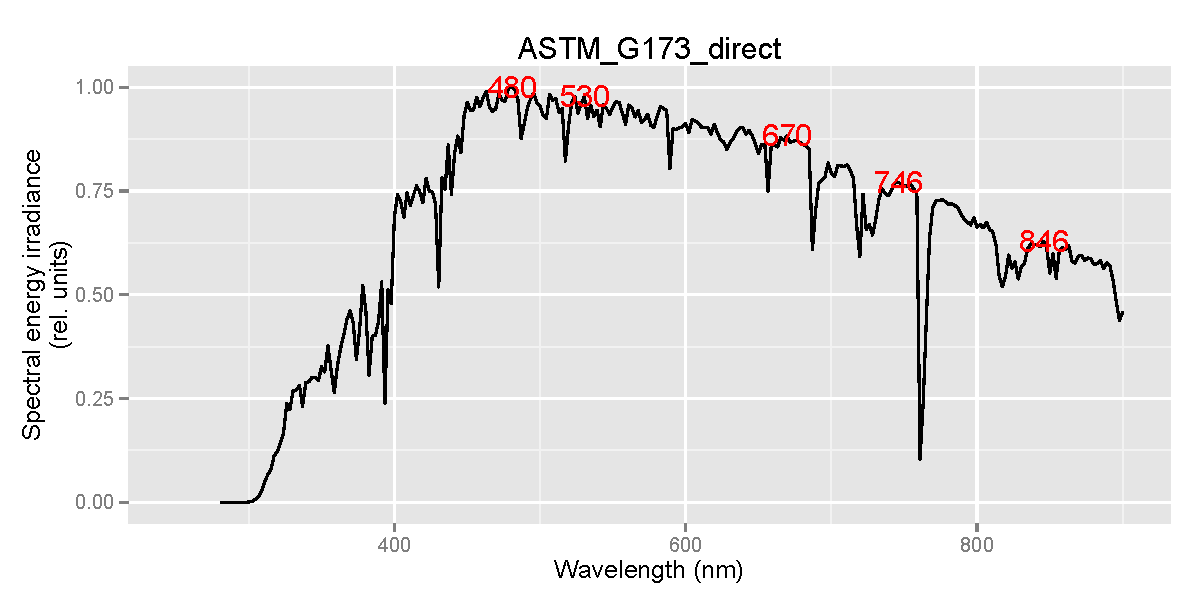
\includegraphics[width=.95\textwidth]{figure/pos-terrestrial-std1} 
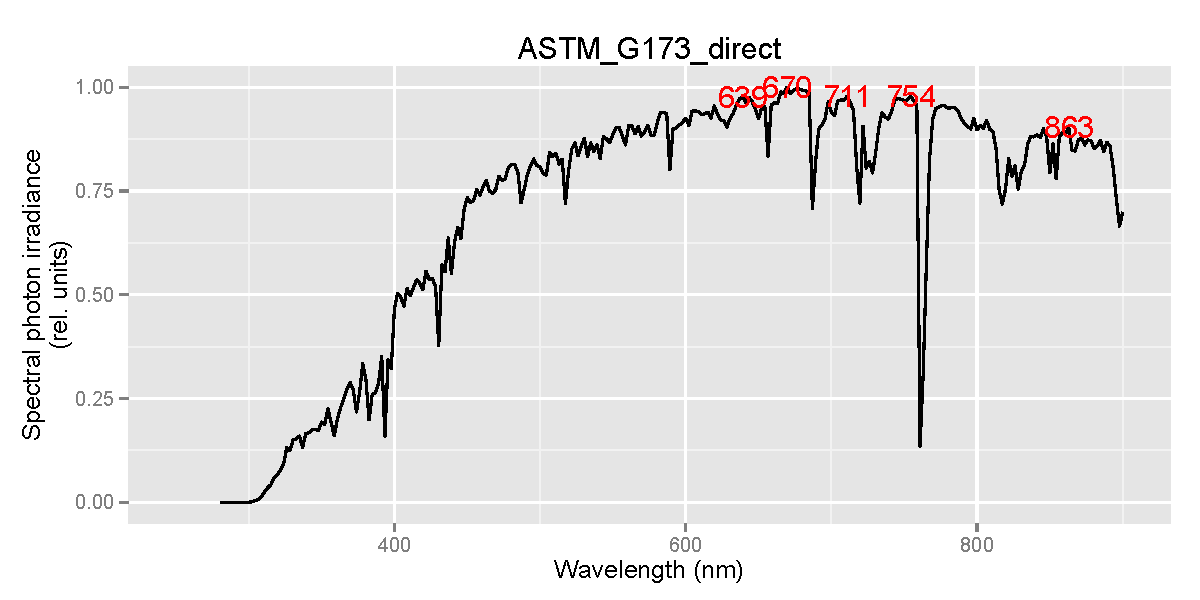
\includegraphics[width=.95\textwidth]{figure/pos-terrestrial-std2} 
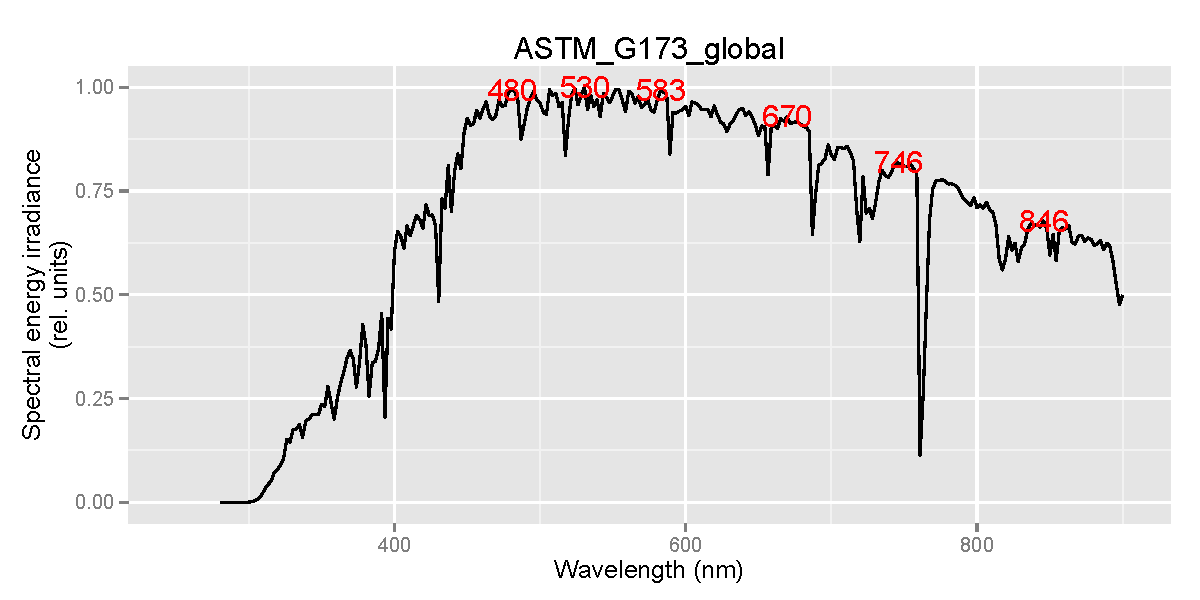
\includegraphics[width=.95\textwidth]{figure/pos-terrestrial-std3} 
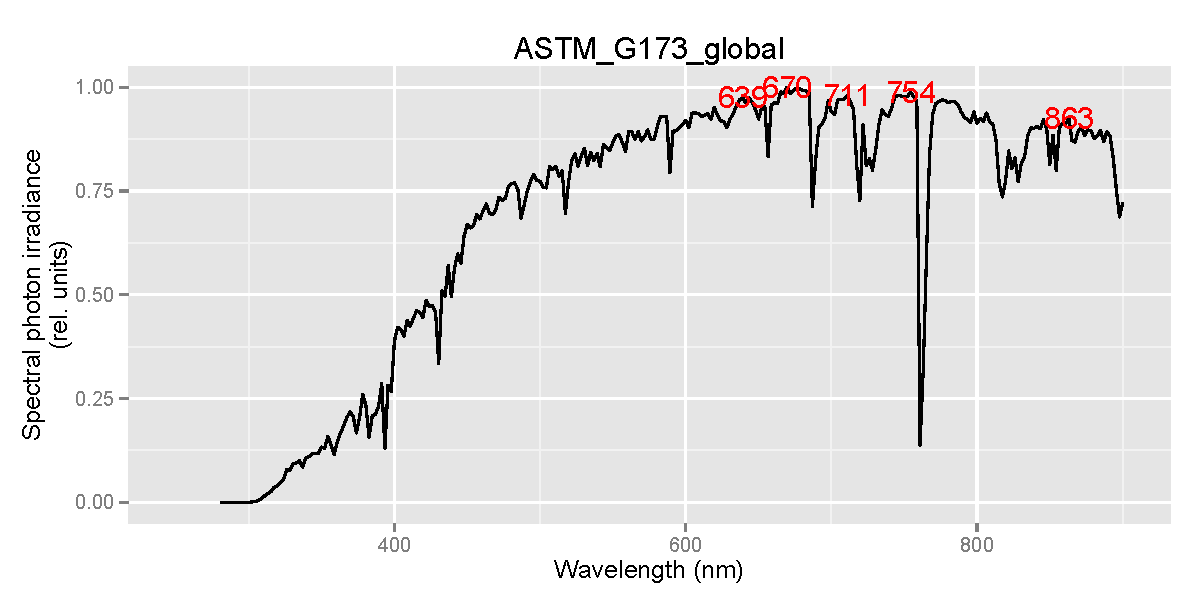
\includegraphics[width=.95\textwidth]{figure/pos-terrestrial-std4} 

}



\end{knitrout}


\section{Measured dayligh spectra}

\begin{knitrout}\footnotesize
\definecolor{shadecolor}{rgb}{0.969, 0.969, 0.969}\color{fgcolor}\begin{kframe}
\begin{alltt}
\hlstd{spectra} \hlkwb{<-} \hlkwd{c}\hlstd{(}\hlstr{"sun_May_morning"}\hlstd{)}
\hlkwa{for} \hlstd{(spc} \hlkwa{in} \hlstd{spectra) \{}
    \hlkwd{lamp.plotter}\hlstd{(}\hlkwc{lamp.name} \hlstd{= spc)}
\hlstd{\}}
\end{alltt}
\end{kframe}

{\centering 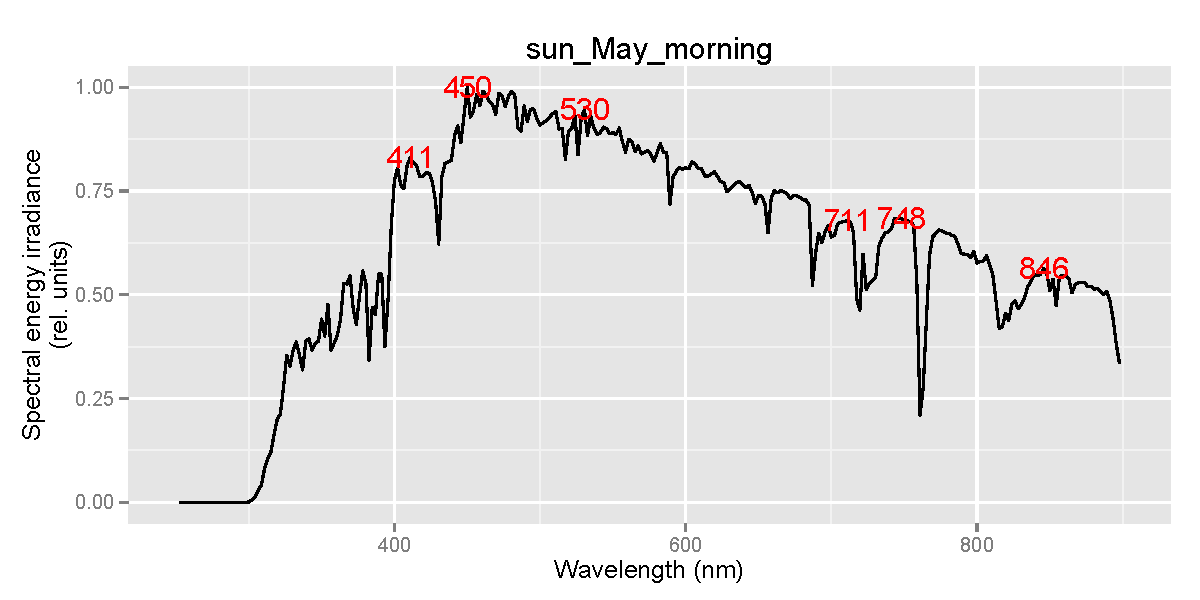
\includegraphics[width=.95\textwidth]{figure/pos-terrestrial-meas1} 
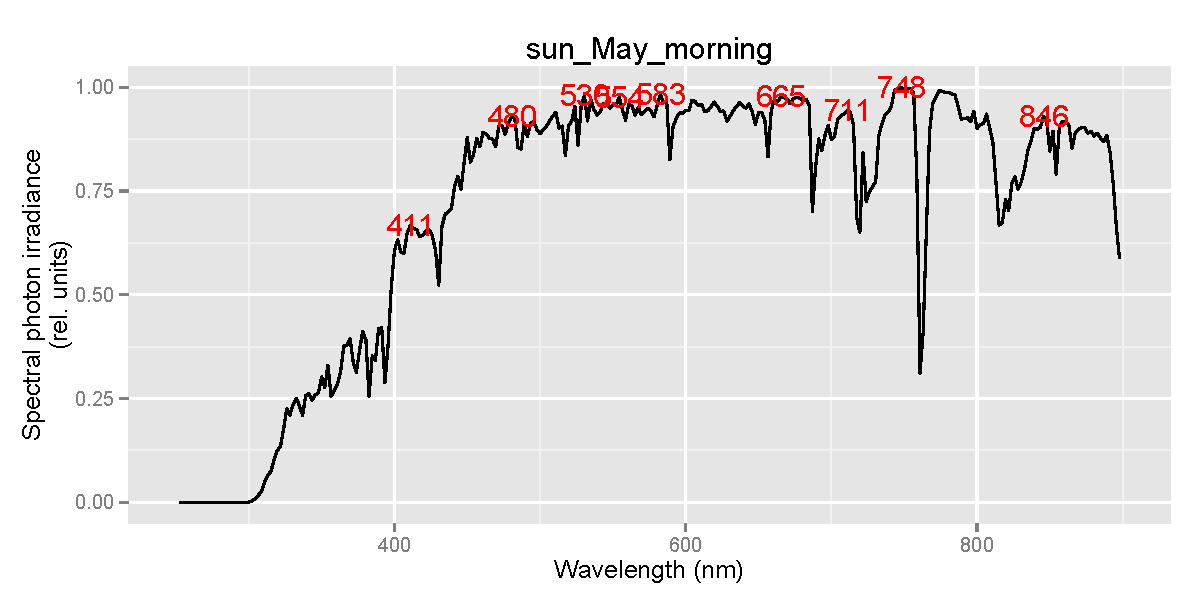
\includegraphics[width=.95\textwidth]{figure/pos-terrestrial-meas2} 

}



\end{knitrout}



\end{document}
